\section{Experiments}
\label{sec:experiments}

We validate the paper's contributions in turn: that public scores can fail to yield a
ranking at all; that Concentration and Invariance each supply evidence a composite score
would erase; that Grounding and Faithfulness's objective-ground-truth readouts (G-VS,
F-3) reach a hazard-judgement-free version of the same dissociation and replicate across
scenario and data source, though less completely than Concentration; and that a
diagnosed causal link can be repaired without a guaranteed behavioural payoff. Every
number is traceable to a released artifact, and every positive finding reported below
has been checked against an explicit attempt to explain it away
(\cref{sec:ablation}).

\subsection{Setup}
\label{sec:setup}

We evaluate six end-to-end driving policies chosen to separate three confounds that a
smaller pool cannot: \emph{encoder family}, \emph{action-head family}, and \emph{native
training domain} (\cref{tab:policies}). LTF, DiffusionDrive and DiffusionDriveV2 share
one \texttt{TransfuserBackbone} encoder under three different action heads (continuous
regression, anchored diffusion, improved anchored diffusion), isolating whether a null
result is caused by the encoder or the head. SimLingo and the two VLAs (Alpamayo-R1,
AutoVLA) provide an architecture-family contrast. A three-way config/weights/output
comparison confirmed that TransFuser and LTF are the identical candidate under this
repository's release (SimScale), so we report LTF only.

\begin{table}[t]
\centering
\caption{Policies under test. $^\dagger$Domain from checkpoint metadata, not independently verified.}
\label{tab:policies}
\scriptsize
\resizebox{\linewidth}{!}{%
\begin{tabular}{lllll}
\toprule
Policy & Encoder & Action head & Input & Domain \\
\midrule
SimLingo & InternVL2-1B, 24L & continuous regression & single-frame & CARLA (sim) \\
DiffusionDrive & TransFuser (ResNet-34$\times$2) & anchored diffusion & single-frame & NAVSIM$^\dagger$ \\
LTF & TransFuser (latent) & continuous regression & single-frame & NAVSIM$^\dagger$ \\
DiffusionDriveV2 & TransFuser (+lidar BEV) & diffusion + PDM select & single-frame & NAVSIM$^\dagger$ \\
Alpamayo-R1 & Cosmos-Reason1, 36L & AR action tokens & multi-frame & PhysicalAI-AV$^\dagger$ \\
AutoVLA & Qwen2.5-VL-3B, 36L & AR action tokens & multi-frame & NAVSIM$^\dagger$ \\
\bottomrule
\end{tabular}}
\end{table}

All readouts for all six policies are produced on one shared stimulus set: a ghost-probe
event corpus (7003 events mined from nuScenes trainval; positive triggers A/B/C for VRU
emergence, close cut-in and generic TTC drop), a geometry-balanced negative system
(caliper-matched harmless statics, used to build F-3's clean/ghost pairing), and
a controlled domain pairing (CARLA rendering vs.\ world-model photorealistic
re-rendering of the same scene, $do(\text{appearance})$, 216 pairs). Every axis is
discovered \emph{and} measured on this one real-domain corpus, never on a candidate's own
training or simulation domain -- the one exception being Invariance, which by definition
requires a real/sim pair. Six input adapters (the dominant engineering cost of this
study) make the corpus isomorphic across architectures; LTF and DiffusionDriveV2 reuse
DiffusionDrive's adapter front end verbatim, which is what makes their pairwise
comparison in \cref{sec:main-results} valid. Concentration is measured on two pairing
sources under the general formula of \cref{sec:method} -- \emph{C-domain} (sim/real
rendering pairs) and \emph{C-hazard} (clean/ghost pairs) -- gated by a patch-ALL
sufficient-cut-set self-check (recovery must fall in $[0.7,1.3]$); a failed self-check
forces an indeterminate verdict regardless of the nominal per-layer numbers.

Statistical discipline is scene-level throughout, one pre-registered primary readout per
experiment, three-state adjudication (PASS/FAIL/\emph{indeterminate}), and
within-model-normalized quantities for every cross-model comparison.

\subsection{Main Results}
\label{sec:main-results}

\paragraph{Public scores do not yield a ranking.} \Cref{tab:public-scores} shows
that even the two best-known candidates report incommensurable numbers -- different
benchmark, domain, protocol and metric. Growing the pool to six does not repair this: of
the six, only four nominally share a NAVSIM PDMS figure, drawn from different splits and
self-reported pipelines we did not re-run, SimLingo has only a CARLA score, and
Alpamayo-R1 has neither. We therefore treat no public score as evidence in what follows;
\cref{tab:main-matrix-v1}, measured on one stimulus set under one protocol, is this paper's
substitute.

\begin{table}[t]
\centering
\caption{Public scores are incommensurable: different benchmark, domain, protocol and metric.}
\label{tab:public-scores}
\scriptsize
\resizebox{\linewidth}{!}{%
\begin{tabular}{lllll}
\toprule
Policy & Benchmark & Metric & Score & Protocol \\
\midrule
SimLingo & CARLA LB2.0 & Driving Score & 6.87 & closed-loop sim \\
DiffusionDrive & NAVSIM navtest & PDMS & 88.1 & non-reactive replay \\
\bottomrule
\end{tabular}}
\end{table}

\paragraph{G-VS and F-3.} We operationalize Grounding and Faithfulness as two readouts
that need no human judgement of ``what counts as dangerous,'' and that apply uniformly
regardless of single- vs.\ multi-frame input or language vs.\ no-language interface:
\textbf{G-VS} asks whether a linear probe on the representation recovers object-ness
segmentation (pseudo ground truth from Segment Anything~\cite{kirillov2023sam}, an
objective, task-independent target); \textbf{F-3} asks whether occluding the hazard
entity at the input causes the action to revert toward its no-hazard baseline (an
input-level necessity intervention, not a representation-level correlation).
\Cref{tab:main-matrix-v1} reports both for all six candidates with no grouping.

\begin{figure}[t]
\centering
\begin{tabular}{cc}
\includegraphics[width=0.47\linewidth]{figures/f3_example/02_ghost_web.jpg} &
\includegraphics[width=0.47\linewidth]{figures/f3_example/03_ghost_occluded_web.jpg} \\
{\scriptsize (i) ghost frame $x_{ghost}$} & {\scriptsize (ii) occluded, $x_{occ}$} \\
\includegraphics[width=0.47\linewidth]{figures/f3_example/04_ghost_sam_overlay_web.jpg} &
\includegraphics[width=0.47\linewidth]{figures/f3_example/01_clean_web.jpg} \\
{\scriptsize (iii) SAM mask of the entity} & {\scriptsize (iv) clean frame $x_{clean}$}
\end{tabular}
\caption{A real F-3 event (nuScenes scene-0862, a pedestrian crossing directly into the
ego's path, $d_{long}=12.2$\,m at emergence). (ii) is the literal input the policy
receives for the necessity arm: the entity's box, filled with the frame's own mean
colour (not a synthetic hole), produced by the same \texttt{occlude()} call used to
compute every $R$ in \cref{tab:main-matrix-v1}. (iii) is for illustration only -- G-VS
and F-3 use SAM independently, on different frames, for different purposes.}
\label{fig:f3-example}
\end{figure}

\begin{table}[t]
\centering
\caption{G-VS / F-3: v1 primary readouts, six candidates, no grouping.}
\label{tab:main-matrix-v1}
\scriptsize
\resizebox{\linewidth}{!}{%
\begin{tabular}{lcccc}
\toprule
Policy & G-VS selectivity & verdict & F-3 necessity $R$ & verdict \\
\midrule
SimLingo & $\mathbf{+0.0273\ [+0.0128,+0.0424]}$ & \textbf{PASS} & $+0.461\ [+0.166,+0.789]$ & indet.\ (CI spans 0.5) \\
DiffusionDrive & $\mathbf{+0.0381\ [+0.0211,+0.0551]}$ & \textbf{PASS} & no baseline response & indeterminate\textsuperscript{1} \\
LTF & $+0.0191\ [-0.0006,+0.0385]$ & indeterminate & $+0.113\ [+0.044,+0.191]$ & \textbf{FAIL}\textsuperscript{2} \\
DiffusionDriveV2 & $+0.0159\ [-0.0029,+0.0353]$ & indeterminate & no baseline response & indeterminate\textsuperscript{1} \\
Alpamayo-R1 & n.m.\textsuperscript{3} & -- & no baseline response & indeterminate\textsuperscript{1} \\
AutoVLA & n.m.\textsuperscript{3} & -- & no baseline response & indeterminate\textsuperscript{1} \\
\bottomrule
\end{tabular}}

\vspace{4pt}
{\scriptsize\textsuperscript{1}The baseline response $b_{ghost}$ is itself indistinguishable from 0: untestable, not a failed test. $b_{ghost}$ contrasts a hazard frame against a pre-emergence frame, in $219/288$ of which the entity is already visible (ghost/clean imaged-area ratio median $1.67$), so it measures a closer approach rather than an appearance. The reading is not an artifact of single-frame sampling: re-running all four arms as the mean of a $9.9$-frame window per event leaves $b_{ghost}$ indistinguishable from 0 for both affected candidates and every verdict in this table unchanged. \textsuperscript{2}Occluding the hazard entity removes only 11\% of the response -- a blind-action signature~\cite{embodiedinterp2026}. \textsuperscript{3}Not measured (video-token layout unresolved for these two), not n/a.}
\end{table}

Two required control arms do real work here. G-VS's \texttt{position\_only} floor (token
coordinates alone, no representation) already reaches mIoU $0.333$ against a trained mIoU of
$0.35$--$0.40$: most of the raw score is a spatial prior, and the representation's net
contribution is only $0.02$--$0.04$. Selectivity (trained $-$ random-init, a control task in
the sense of \citet{hewitt2019designing}) is a paired difference and remains credible despite
the small net contribution. F-3's control arm $R_{ctrl}$ (an equal-area grey patch placed
elsewhere in the frame) falls in $[-0.09,+0.16]$ with CIs spanning 0 for all six candidates --
occlusion by itself does not return the action to baseline, which is the precondition for
LTF's FAIL to mean what it says.

\textbf{The most informative cell is DiffusionDrive}: the highest G-VS selectivity in the
table ($+0.038$, its representation does carry object-ness information) paired with an F-3
baseline response indistinguishable from zero (its action does not react to hazard frames
at all, and still does not under a $9.9$-frame window average). Seeing and acting on it are
independent, without any judgement of what counts as dangerous. Its action is not inert:
under the window average, erasing the entity within a frame does move its planned speed
($-0.0084\,[-0.0155,-0.0026]$), but by no more than painting an equal-area patch elsewhere
does ($\lvert d_{occ}\rvert-\lvert d_{ctrl}\rvert = -0.0012\,[-0.0069,+0.0037]$) -- a
sensitivity to the perturbation, not to the hazard.

\paragraph{G-VS and F-3 generalize across a structurally different scenario and an
independently collected data source.} All results above are measured on one ghost-probe
corpus mined from nuScenes. We test portability along two independent axes: a
structurally different scenario (an already-tracked lead vehicle braking hard, rather
than a new entity entering the path, for SimLingo, DiffusionDrive and LTF) and an
independently collected data source (NAVSIM's underlying OpenScene/nuPlan logs, with
velocity from tracked 3D boxes rather than finite-differenced, at up to 397 positives, a
larger sample than the discovery corpus, for four candidates). \Cref{tab:generality}
summarizes every axis re-measured on both.

\begin{table}[t]
\centering
\caption{Portability across a structurally different scenario (lead-vehicle braking) and
an independently collected data source (NAVSIM).}
\label{tab:generality}
\scriptsize
\resizebox{\linewidth}{!}{%
\begin{tabular}{lll}
\toprule
Axis & Scenario-generality & Data-source-generality \\
\midrule
C & 6/6 cells match & 8/8 cells match \\
G-VS & verdict 1/4; pt.\ est.\ 4/4 in band\textsuperscript{1} & verdict 2/4; pt.\ est.\ 4/4 in band\textsuperscript{1} \\
F-3 & untestable $\times$6\textsuperscript{2} & LTF FAIL replicates; no-response 3/3 \\
\bottomrule
\end{tabular}}

\vspace{4pt}
{\scriptsize\textsuperscript{1}All 12 G-VS selectivity point estimates, across three corpora and four candidates, fall in $[+0.016,+0.041]$. \textsuperscript{2}F-3's primary criterion (necessity ratio $R$, gated on a significant $b_{ghost}$) adjudicates all six candidates indeterminate here. That corpus tracks the lead vehicle throughout, so its clean arm is not hazard-absent: the entity projects visible in the clean frame in $103/103$ events at unchanged imaged size (ghost/clean area ratio median $1.00$), and $b_{ghost}$ contrasts braking onset rather than entity presence. A supplementary within-frame contrast that does not use the clean arm, $d_{occ}=v_{plan}(\text{ghost})-v_{plan}(\text{occ})$, is significant, specific and correctly signed for SimLingo ($-0.510\,[-0.736,-0.307]$; control $-0.032\,[-0.117,+0.048]$) and LTF ($-0.028\,[-0.047,-0.011]$; control $+0.007\,[-0.001,+0.016]$). It supplies no denominator for $R$ and does not change the PASS threshold, so ``untestable'' here refers to the necessity ratio, not to the absence of any occlusion response.}
\end{table}

\textbf{Concentration replicates completely}: 14 of 14 cells agree in
architecture-conditioned sign, responsible layer, and commitment-layer presence/absence
across both tests, including a pre-registered held-out prediction (all three
TransFuser-family members show an interior peak, all three pure-transformer stacks
cascade, confirmed before the third pure-transformer candidate, SimLingo, was measured)
and a candidate-specific self-check failure (DiffusionDriveV2's patch-ALL gate) that
travels with the candidate rather than the corpus ($0.552\to0.642$, both indeterminate).

\textbf{G-VS's point estimate is stable, its three-state verdict is not.} Across three
corpora (discovery, lead-braking, NAVSIM) and four candidates, all 12 measured
selectivity values fall in a narrow band, $+0.016$ to $+0.041$, with no sign flips and no
collapse toward zero; only SimLingo's three verdicts agree (PASS throughout), while the
other three candidates' PASS/indeterminate calls change across corpora because the effect
size and the CI half-width are the same order of magnitude. On NAVSIM specifically, the
\texttt{position\_only} floor exceeds trained mIoU for two candidates (SimLingo $0.4108$
vs.\ $0.4075$; DiffusionDriveV2 $0.3711$ vs.\ $0.3551$) -- a property of that corpus's more
regular object placement, not of any model -- which does not invalidate the paired,
random-init-relative selectivity readout but narrows what a PASS supports: object-ness
information above a random-init floor, not a claim that the representation is more useful
than knowing token position.

\textbf{F-3's most portable finding is negative.} Four candidates (DiffusionDrive,
DiffusionDriveV2, and, on the corpora where they were tested, Alpamayo-R1 and AutoVLA)
show no detectable baseline response to a hazard frame at all, on every corpus tested
(3/3, 3/3, 2/2, 2/2) -- the single most robust finding in this study. Where a baseline
response does exist, F-3's verdict replicates cleanly: LTF's blind-action signature
reproduces on NAVSIM with an almost identical response magnitude ($b_{ghost}=-0.0245$ on
the discovery corpus vs.\ $-0.0249$ on NAVSIM) and an even lower necessity ratio
($R=+0.113\to+0.008$), while its control arm stays centered on zero on both corpora. F-3's
necessity ratio could not be evaluated on the lead-braking corpus for either candidate
with a signature elsewhere (SimLingo, LTF), because neither shows a baseline response
there -- a structural limitation of a necessity test (it is only testable where a
candidate reacts at all), not a failure of the method. On that corpus the limitation is
partly definitional: the lead vehicle is tracked throughout, so the clean arm is not
hazard-absent (the entity projects visible in $103/103$ clean frames, at a ghost/clean
imaged-area ratio of median $1.00$), and $b_{ghost}$ there contrasts braking onset rather
than entity presence. A within-frame contrast that bypasses the clean arm shows that both
candidates do respond to occluding the lead vehicle, significantly and specifically
(SimLingo $-0.510\,[-0.736,-0.307]$, LTF $-0.028\,[-0.047,-0.011]$, both control arms
centered on zero); it supplies no denominator for $R$ and so leaves the verdict unchanged.

G-VS and F-3 are thus more portable than the semantic-construct readouts they replace --
neither collapses in point estimate or reverses sign -- short of Concentration's
consistency; both have a narrower, diagnosable failure mode (a borderline verdict, or an
untestable baseline) instead.

\paragraph{C: one diagnostic prescribes two different repairs, and generalizes into a
held-out-confirmed architectural law.} On the same rendering-domain pairing,
SimLingo's recovery profile decreases monotonically from L0 (1.004) to L23 (0.000,
Spearman $-0.997$): the failure has already entered at the vision-to-LLM interface.
DiffusionDrive is the opposite -- L0/L1 recovery is near zero with an interior peak at L6
(Spearman $+0.929$ under the clean/ghost pairing) -- so the two policies require repairs
at entirely different sites, information \cref{tab:public-scores} structurally cannot
contain. Switching the pairing source from sim/real rendering to clean/ghost (C-hazard)
lets the same method ask a different question, and it converges: DiffusionDrive and LTF,
which share one encoder, both localize hazard-induced change to L6 ($C_m$ $0.801$ and
$0.789$) -- the only concordant diagnosis among architecturally distinct pairs in this
study.

\emph{Causal responsibility is not the same quantity as the strength of a correlational
proxy, and the two disagree on where to intervene.} On DiffusionDrive's sim/real
pairing, the two most natural correlational stand-ins for ``where the domain shift
matters'' -- attention-map JS divergence and $1{-}\mathrm{CKA}$ -- both peak at L7, and
L7 has almost the lowest causal recovery of any layer (\cref{fig:tsne}, silhouette-based
separability of sim vs.\ real activations peaks at yet a third layer, L5). All three
proxies disagree with each other and with the true causal peak at L6. ``Intervene where
the representation changes most'' -- the intuition a correlational diagnostic
invites -- would place a repair at L7 or L0, exactly the sites this axis's own causal
readout rules out.

\begin{figure}[t]
\centering
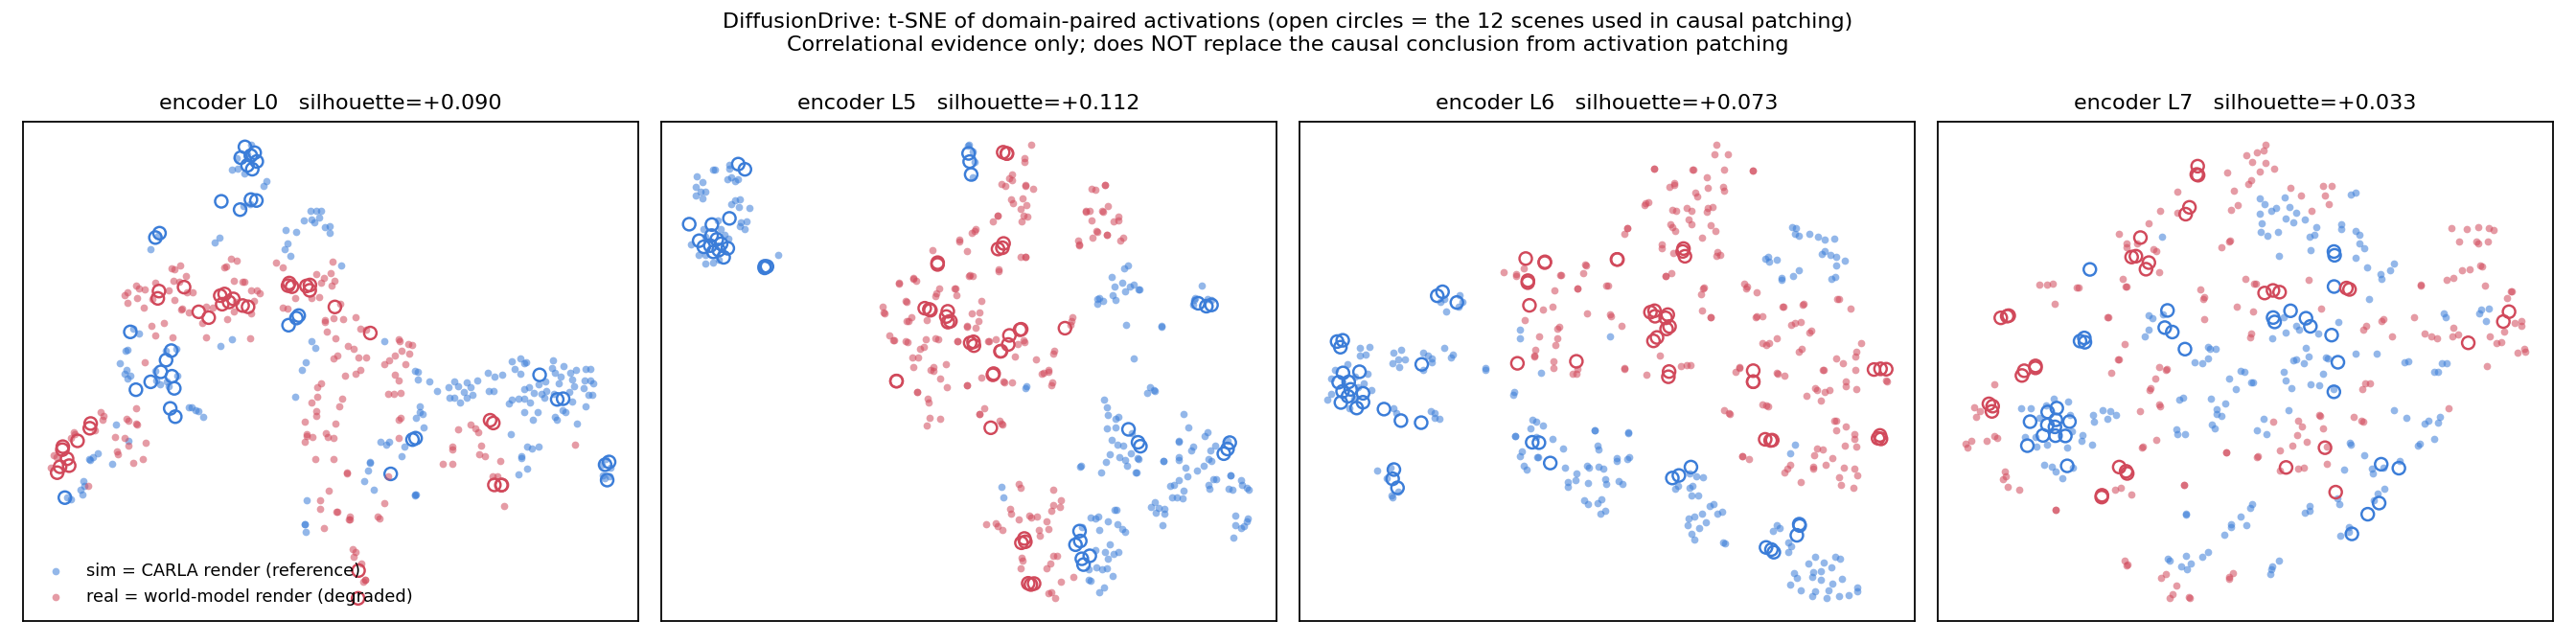
\includegraphics[width=\linewidth]{figures/c_axis_tsne.png}
\caption{t-SNE of DiffusionDrive's per-layer activations, sim (CARLA render) vs.\ real
(world-model render), for four representative encoder layers; open circles are the 12
scenes used in causal patching. Separability (silhouette) peaks at L5, divergence (JS,
$1{-}\mathrm{CKA}$) peaks at L7, and the causal peak is L6 -- three distinct quantities,
three different answers. Correlational only; it does not substitute for the causal
verdict in \cref{sec:main-results}.}
\label{fig:tsne}
\end{figure}

This pattern generalizes into a pre-registered, held-out-confirmed law. Having observed a
cascade on the two pure-transformer VLAs (Alpamayo-R1, AutoVLA) and an interior peak on
two TransFuser-family members, we registered the prediction that \emph{any} pure-transformer
stack's C-hazard profile must cascade \emph{before} measuring the third and structurally
different pure-transformer candidate, SimLingo -- a genuine held-out test, not a
redescription of existing data. It confirms exactly: all three TransFuser-family members
(DiffusionDrive, LTF, DiffusionDriveV2) show an interior peak (Spearman $+0.93,+0.93,+0.81$,
committing by L4--L6 of 8), and all three pure-transformer stacks (SimLingo,
Alpamayo-R1, AutoVLA) cascade (Spearman $-0.997,-0.873,-0.859$) -- a clean split with no
sign overlap across six independent candidates. One sub-claim of the original prediction
was too strong and we do not soften it: it held that a pure-transformer profile must
plateau near 1.0 through its early layers, but SimLingo's decline is gradual rather than
a plateau, so its commitment layer arrives at relative depth $0.17$ against
$0.47$ and $0.58$ for the two VLAs. The qualitative direction of the failure's entry
point is architecture-determined; how quickly it decays is not. DiffusionDriveV2's
nominal C-hazard ($C_m=0.845$, the highest of any candidate) has a patch-ALL self-check
that returns $0.552$, far from the required sufficient-cut-set range: the
highest-looking number in the pool is exactly the one our own gate forces us to
withhold.

\paragraph{A representation-steering diagnosis feeding the pilot intervention.} On
SimLingo, we identify the model's causally-effective braking-control direction
$v_{brake}$ via a per-layer activation-injection sweep (adding a scaled unit vector to the
residual stream and reading the resulting change in planned speed), validated against an
in-house upper-bound axis (the model's own braking residual, effective by construction)
and an independent analytic Jacobian cross-check (agreement within 7\% at deep layers,
event-level $r=+0.993$). Injecting along $v_{brake}$ moves planned speed with slope
$-0.0405$, while SimLingo's driving-query representation linearly decodes
time-to-collision (held-out $r=+0.320$) along a direction whose cosine to $v_{brake}$ is
$-0.005$ -- geometrically unrelated. Hazard information is present and the braking
pathway is causally effective, but the two are not connected; \cref{sec:future} extends
this test to the pool.

\paragraph{I: domain robustness resists compression into one number, on both axes
of comparison.} On the same rendering pairing, the representational readout ranks
SimLingo above DiffusionDrive ($I_m$ $0.606$ vs.\ $0.203$) while the behavioural
domain-sensitivity readout ranks them in the opposite order ($0.115$ vs.\ $0.346$), with
non-overlapping CIs on both sides -- any single number must discard one ordering.
Extending the comparison to LTF, which shares DiffusionDrive's exact encoder
architecture under different weights, shows the readout is a property of the trained
weights rather than the architecture ($I_m$ $0.583$ vs.\ $0.203$); a layer-matched
self-check confirms this ordering holds only at each model's own peak layer and reverses
at L0--L4, a qualification we keep in the main text because it is precisely what
distinguishes a diagnostic axis from a robustness score.

\paragraph{Intervening on the diagnosed link.} Guided by the representation-steering
diagnosis above, we post-trained only SimLingo's 229k-parameter
\texttt{speed\_wps\_head} (everything else frozen) with a loss whose coupling term is
exactly $\cos(g,\hat v_{brake})$, so the repaired quantity and the verification quantity
coincide.
\Cref{tab:pilot} includes an attribution-control arm (A1: task loss only, no coupling).

\begin{table}[t]
\centering
\caption{Pilot post-train on SimLingo (229k parameters), held-out scenes.}
\label{tab:pilot}
\scriptsize
\resizebox{\linewidth}{!}{%
\begin{tabular}{lccc}
\toprule
Arm & b-AUC [95\% CI] & $\Delta_{1\sigma}$ [m/s] & $\cos(g,\hat v_{brake})$ \\
\midrule
A0 (untrained) & $0.544\ [0.461,0.621]$ & $+0.091$ & $+0.046$ \\
A1 (task only) & $0.592\ [0.496,0.680]$ & $-0.076$ & $-0.016$ \\
A2 (task+coupling) & $0.593\ [0.499,0.679]$ & $\mathbf{-0.301}$ & $\mathbf{-0.068}$ \\
\bottomrule
\end{tabular}}
\end{table}

The coupling is decisively repaired ($\Delta_{1\sigma}$ flips sign, a factor of 3.3), but
the behavioural score's apparent gain (A2$-$A0 $=+0.051$) is almost entirely explained by
the task-only control (A1$-$A0 $=+0.050$; A2$-$A1 $=+0.001\ [-0.004,+0.007]$). Both halves
of this result matter together: the diagnosed causal link can genuinely be repaired, and
at this budget, repairing it does not translate into a behavioural gain.

\paragraph{Why we report a matrix, not a score.} The four axes differ in units and
adjudication state cell by cell: G-VS and F-3 are within-model-normalized and align
across models but only where a baseline response is measurable; C's formula is invalid
wherever its interior-peak premise fails; I's two readouts can order the same pair of
models oppositely. No candidate dominates on every measurable axis, and a substantial
share of cells across \cref{tab:main-matrix-v1,tab:generality} adjudicate as
indeterminate or not measured, for structurally different reasons (missing stimulus
modality, a violated operationalization premise, an instrument without resolving power,
insufficient statistical power, or a failed self-check). Weighting them into a scalar
would require an unjustifiable imputation decision for each such cell and would make the
provenance of any resulting rank untraceable; we report the matrix instead.

\subsection{Validity Checks}
\label{sec:ablation}

\Cref{tab:validity} summarizes six checks, each designed to rule out one specific way a
result in \cref{sec:main-results} could look real but mean nothing. All six numbers
reported are final.

\begin{table*}[t]
\centering
\caption{Validity checks: what each rules out, and the final verdict.}
\label{tab:validity}
\footnotesize
\begin{tabular}{p{0.19\textwidth}p{0.40\textwidth}p{0.315\textwidth}}
\toprule
Check & What it rules out & Verdict \\
\midrule
In-house upper-bound axis (model's own braking residual, effective by construction) & Attributing a null injection result to the specimen rather than the instrument & SimLingo's instrument is valid (slope $-0.0405$); DiffusionDrive's, LTF's and DiffusionDriveV2's all fail even this by-construction axis $\Rightarrow$ null is instrument-side, localized to the shared TransFuser encoder, not to any one action head \\
Analytic Jacobian cross-check & An empirical injection slope being a measurement artifact & Matches empirical measurement to within 7\% at deep layers (event-level $r=+0.993$); systematically diverges at shallow/mid layers, quantifying where the empirical sweep is required \\
Recovery-profile shape diagnostic & Applying $C_m$ where its interior-peak premise is violated & SimLingo's profile is a monotone cascade ($\rho=-0.997$); reading its $C_m$ literally would misreport a null as a concentrated failure \\
Attribution control (task-only arm, pilot) & Crediting a targeted intervention for a gain produced by the baseline objective alone & 98\% of the pilot's apparent behavioural gain is attributable to task fine-tuning alone, not to the coupling term \\
Full-population null enumeration vs.\ Gaussian-tail extrapolation & Under-estimating a multiple-comparison threshold in an argmax-over-116k search & Empirical 99.9th percentile is up to an order of magnitude above the Gaussian estimate; the number of ``doubly corroborated'' directions drops from 11 to 0 once corrected \\
F-3 occlusion completeness and temporal sampling (per-frame projection across the input window; non-camera sensor channels; one frame vs.\ a window average) & An F-3 necessity reading produced by an occlusion that leaves the entity present in the model's input & The entity projects into a mean of $4.00/4$ window frames for Alpamayo-R1 and $3.44/4$ for AutoVLA, and into the lidar returns of the one point-cloud-consuming candidate (median 1 point at a median range of $27$\,m); occluding every frame into which it projects and deleting the returns inside its 3D box, with the control arm treated symmetrically throughout, leaves all three affected verdicts unchanged. $b_{ghost}$ is unaffected by construction and the lidar channel contributes $\Delta b_{occ}=+0.005\ [-0.004,+0.015]$, so the F-3 readings of \cref{tab:main-matrix-v1} do not rest on the completeness of the occlusion. Re-running all four arms as the mean of a $9.9$-frame window per event, on the four single-frame candidates, likewise leaves every verdict unchanged (CI half-width ratios $0.45$--$1.11$), so they do not rest on single-frame sampling either \\
\bottomrule
\end{tabular}
\end{table*}

Two of these checks produced a correction substantial enough to change a claim elsewhere
in the paper, not merely a number. First, the in-house-calibration check's original
corollary held that injection effect size is incomparable \emph{across action-head
families}; extending the pool to three models sharing one encoder under two different
heads falsifies this -- all three are unmeasurable regardless of head -- and relocates
the boundary to the \emph{encoder}, which is the version reported in
\cref{sec:main-results}. Second, the shape diagnostic is why DiffusionDriveV2's
highest-looking C-hazard number (\cref{sec:main-results}) is reported as indeterminate
rather than best: its patch-ALL self-check fails, so the per-layer shares underlying that
number are uninterpretable regardless of their face value.

\subsection{Limitations}

(1) The three-way comparison of \cref{sec:intro} is not fully closed, in two senses.
First, our pilot establishes that a diagnosed link is measurable, non-redundant, and
intervenable, not that axis scores predict post-training gains at scale. Second, and more
fundamentally, \cref{fig:pipeline}'s ``real deployment rank'' is in this paper approximated
by pseudo-closed-loop scoring on held-out nuScenes events, not by an actual on-vehicle
closed-loop trial. A real-vehicle deployment study -- collecting on-road ghost-probe
footage, capturing every candidate's intermediate representations at native inference
frequency across all readable layers during on-vehicle inference, and pairing each
capture with a 3D-Gaussian-Splatting reconstruction of the identical physical scene
replayed offline through the same frozen weights -- is in progress but not complete, and
no result from it appears in this paper. Because this study's timeline is independent of
our own, we deliberately do not make the paper's central claim depend on it. We instead
pre-register the analysis before any such data is collected: (i) the C-axis architectural
split of \cref{sec:main-results} should replicate under the real/3DGS pairing; (ii) the
F-axis causal-confusion signature should persist for candidates that already exhibit it
offline; (iii) the I-axis representational/behavioural orderings should agree in
direction, if not magnitude, with those obtained on the CARLA/world-model pairing used
throughout this paper; and (iv) cross-model rankings computed offline (this paper) and
on-vehicle (future work) should correlate positively -- the central claim this whole
protocol is meant to support. Neither the real-vehicle study nor the 3DGS pairing is
reported as a result in this version of the paper.
(2) The scenario-generality test (\cref{tab:generality}) covers three candidates for
Concentration (SimLingo, DiffusionDrive, LTF) and four for G-VS/F-3 (adding
DiffusionDriveV2); Invariance was not re-measured, since its domain pairing is an asset
independent of scenario type. (3) The data-source-generality test, on NAVSIM's underlying
OpenScene/nuPlan logs, is not power-limited relative to the discovery corpus (397
positives, a larger sample), so its results are not an artefact of sample size; it has
its own scope limits, though: the two corpora are not geographically disjoint (a disjoint
subset is reported and agrees), imaging geometry differs across corpora so only
within-corpus contrasts are used, and only NAVSIM's test split (147 logs) was drawn,
leaving room to scale up. (4) G-VS covers only 4 of 6 candidates (the two VLAs' video-token
layout is unresolved, \cref{sec:future}); F-3 is measurable only where a candidate shows
any baseline response to a hazard frame, which is itself the majority verdict across the
pool. (5) C's top-2-share formula ($C_m$) is invalid on profile shapes without an
interior peak (monotone-cascade or self-check-failing profiles) -- an operationalization
boundary, not a statement that a model is weak on that axis. (6) The Invariance axis is
measured on only half the pool because three candidates' native inputs (lidar,
multi-frame history) are absent from the domain-paired corpus, a stimulus-side gap, and
the ordering we do report holds only at each model's own peak layer. (7) The
representation-steering diagnosis behind the pilot intervention is reported only for
SimLingo: the random-direction control has no resolving power at this sample size for the
other candidates (even the by-construction-effective $v_{brake}$ fails to exceed its own
null there), which must not be read as evidence of no causal effect for them. (8) The
domain pairing is a same-geometry dual rendering, not a 3DGS reconstruction, and five of
six candidates' native training domains are inferred from checkpoint metadata rather than
independently verified.

\subsection{Future Work}
\label{sec:future}

The v1 readouts of \cref{tab:main-matrix-v1} cover only the \emph{blind-action} branch of
a three-way taxonomy of VLA failure modes~\cite{embodiedinterp2026}; two further branches,
plus a semantic extension of G-VS, are left for follow-up work.

\paragraph{G-VL: semantic segmentation consistency.} G-VS is binary object-ness --
\emph{where} an object is, not \emph{what} it is. G-VL would replace the
\{background, object\} label space with real semantic classes (pedestrian, vehicle,
static obstacle, drivable area) and test whether category, not merely location, is
linearly readable. The TransFuser family's built-in BEV semantic head (7 classes) is a
ready anchor but lives in BEV space and covers only half the pool, so G-VL needs an
image-space class-labelled ground truth (SAM plus class labels, or an open-vocabulary
segmentation model). It would also settle whether this round's small net contribution
($0.02$--$0.04$ mIoU) reflects sparse information or merely the coarseness of a binary
task.

\paragraph{F-1: post-hoc rationalization.} For the language-producing candidates
(SimLingo, Alpamayo-R1, AutoVLA), test whether Chain-of-Causation text is consistent with
the evidence that actually drives the action: if occluding an entity leaves the action
unchanged (an F-3 FAIL) while the language still asserts a causal story referencing that
entity, the language is post-hoc rationalization, not an explanation of the true
cause~\cite{embodiedinterp2026}. F-1 only becomes informative once some
language-producing candidate clears F-3's baseline-response floor, which none did this
round.

\paragraph{F-2: localizing the true driver.} F-3 shows only that an entity is \emph{not}
what drives the action, not what is. Two priors from the causal-inversion
framework~\cite{samsami2021causal} suggest where to look: \emph{inertia} (the action
follows the ego's own speed history rather than the scene) and \emph{collision} (the
action follows global scene statistics rather than any single entity). A workable design
permutes or freezes the ego speed history and compares the resulting action change
against F-3's ghost-frame response, and repeats the necessity test at the level of
high-attention tokens rather than the hazard entity's box. LTF -- this round's only F-3
FAIL, and so the only confirmed case of ``a response wired to the wrong evidence'' -- is
the candidate to run this on first.
